\documentclass[12pt]{article}
\usepackage{indentfirst}
\usepackage[top=1.0in, bottom=0.8in, left=0.6in, right=0.6in]{geometry}
\usepackage{fourier} % Use the Adobe Utopia font for the document - comment this line to return to the LaTeX default
\usepackage[scaled=0.875]{helvet}
\usepackage{mathtools,amsfonts,amsthm,amssymb} % Math packages
\usepackage{bm}
\usepackage{graphicx}
\usepackage{comment}
\usepackage{hyperref}
\usepackage{xcolor}
\usepackage{color}
\usepackage{transparent}
\usepackage{microtype} % improves the spacing between words and letters.
\setlength\parindent{0.5cm}%indent
\usepackage{setspace} % Change line stretch
\usepackage{framed} 
\usepackage{sectsty} % Allows customizing section commands
\usepackage{fancyhdr} % Custom headers and footers
\setlength{\headheight}{13.6pt} % Customize the height of the header
\usepackage[english]{babel}
\usepackage{cite}
\usepackage{multicol}
\usepackage{listings}
\definecolor{backcolour}{rgb}{0.95,0.95,0.92}
\lstdefinestyle{mystyle}{backgroundcolor=\color{backcolour},commentstyle=\color{olive}, keywordstyle=\color{red}, numberstyle=\tiny\color{gray}, stringstyle=\color{blue}, basicstyle=\footnotesize, breakatwhitespace=false,         breaklines=true,                 captionpos=b,keepspaces=true,numbers=left,numbersep=5pt,showspaces=false,showstringspaces=false, showtabs=false,tabsize=4 } 
\lstset{style=mystyle}
%\usepackage{natbib} %Import the natbib package and sets a bibliography  and citation styles
%\bibliographystyle{apalike}
\begin{document}
% --------------------------------------------------------------
%                        Head 
% --------------------------------------------------------------
\title{Solution of 2-8 sections' last question in\\ Nonlinear Programming\\
    3rd ed, Bazaraa et.}
\author{C }
\maketitle
\section*{Introdution}
This is the trial solutions to the Book
NONLINEAR PROGRAMMING,3rdEd, M.S. Bazaraa et.

Due to the limitation of time, only the first 8 section has been read and 
hence there would be only offered the 2-8 sections' last question for each section.
\section*{2.57}
A 3 dimension plane L and its orthogonal complement (a line). 

\[
    L^{\perp}=z[2,1,-1]^T = z'6^{-0.5}[2,1,-1]^T
\]
\[
    \lambda_2= [1,2,3]\ 6^{-0.5}[2,1,-1]^T =6^{-0.5}
\]
\[
    \bm x_2= 6^{-0.5}*6^{-0.5}[2,1,-1]^T =\frac{1}{6}[2,1,-1]^T
\]
\[
    \bm x_1=\bm x-\bm x_2= [1,2,3]^T-\frac{1}{6}[2,1,-1]^T=\frac{1}{6}[4,11,19]^T
\]
\section*{3.73}
This is about Rvacev Function.

(a)This question is similar to 3.72, there are of course many ways to solve.
Without losing generality, set  $g_1(x)\geq g_2(x)$.
\\
(a: method I)\\
\begin{align*}
G_\alpha(\bm x)&=\frac{1}{2} g_1(\bm x) +\frac{1}{2} g_2(\bm x)
        +\frac{1}{2}\sqrt{ g_1^2(\bm x)+ g_2^2(\bm x)-2\alpha g_1(\bm x)g_2(\bm x) } \\
        &=\frac{1}{2} g_1(\bm x) +\frac{1}{2} g_2(\bm x)
        +\frac{1}{2}\sqrt{ ( g_1(\bm x)- g_2(\bm x) )^2+2(1-\alpha) g_1(\bm x)g_2(\bm x) } 
        \\
        &\geq\frac{1}{2} g_1(\bm x) +\frac{1}{2} g_2(\bm x)
        +\frac{1}{2} ( g_1(\bm x)- g_2(\bm x) )=g_1(\bm x)
\end{align*}

For  $g_2(\bm x)\ge 0$, we could get $g_1(\bm x)\ge 0, G_{\alpha}\ge0$,

For  $g_2(\bm x)< 0$, we could get only when $g_1(\bm x)\ge 0$,
$\frac{1}{2}\sqrt{ ( g_1(\bm x)- g_2(\bm x) )^2+2(1-\alpha) g_1(\bm x)g_2(\bm x) } 
\le \frac{1}{2} ( g_1(\bm x)- g_2(\bm x) )$, so that $G\ge 0$.
Otherwise,$g_1(\bm x)<0 $,
$\frac{1}{2}\sqrt{ ( g_1(\bm x)- g_2(\bm x) )^2+2(1-\alpha) g_1(\bm x)g_2(\bm x) } 
\ge \frac{1}{2} ( g_1(\bm x)- g_2(\bm x) )$, so that $G< g_1(\bm x)< 0$.

Therefore,
\[
\min G_\alpha(\bm x) =  0\Leftrightarrow g_1(\bm x) \ge 0
\]

(a: method II)\\
For the Prime Problem:
\begin{align*}
    \min G_\alpha(\bm x)&\\
    -g_1 (\bm x)&\leq0\\
    \bm x &\in \bm X
\end{align*}
Its Lagrangian Dual Problem would be:
\begin{align*}
    \max \theta( \mu)&\\
     \mu &\geq  0\\
    \theta(\mu)&=\inf\{
        G_\alpha(\bm x)-\mu g_1(\bm x)
        ,
    \bm x \in \bm X
    \}
\end{align*}
%Since we could let $\mu$ to be infinitely large, 
\[
    \theta(\mu)=\inf\{
        (\frac{1}{2}-\mu_1 ) g_1(\bm x) +\frac{1}{2} g_2(\bm x)
        +\frac{1}{2}\sqrt{ g_1^2(\bm x)+ g_2^2(\bm x)-2\alpha g_1(\bm x)g_2(\bm x) }
        , \bm x \in \bm X \}
        %~~~~~~~(\bm\mu\rightarrow \infty)
\]
Then to get the $\inf$, $g_1$ would be 0,
$\theta(\mu )=0$. As $g_1(\bm x)=0$, the only restrict of Prime Problem is constraining, so
this would no be a saddle point. Therefore:
\[
\min G_\alpha(\bm x) = 0 \Leftrightarrow \max\theta = 0\Leftrightarrow g_1(\bm x) \ge 0
\]

(b)
For each $\alpha$, 
\begin{align*}
G_\alpha(\bm x)&=
\frac{1}{2} g_1(\bm x) +\frac{1}{2} g_2(\bm x)
        +\frac{1}{2}\sqrt{ g_1^2(\bm x)+ g_2^2(\bm x)-2\alpha g_1(\bm x)g_2(\bm x) } \\
&=
\frac{1}{2} g_1(\bm x) +\frac{1}{2} g_2(\bm x)
        +\frac{1}{2}\sqrt{ ( g_1(\bm x)-\alpha g_2(\bm x) )^2+(1-\alpha^2)g_2(\bm x) } 
\end{align*}

Set $cos\theta= -\alpha, \theta\in [\frac{1}{2}\pi,\pi]$, we could rewrite $G$ as:
\begin{align*}
G_\alpha(\bm x)&=
\frac{1}{2} g_1(\bm x) +\frac{1}{2} g_2(\bm x)
        +\frac{1}{2}\sqrt{ ( g_1(\bm x)-\cos\theta g_2(\bm x) )^2+\sin^2\theta g_2(\bm x) } 
%G_\alpha(\bm x)&=
%c g_3(\bm x) +d g_4(\bm x)
        %+\frac{1}{2}\sqrt{ g_3^2(\bm x)+ g_4^2(\bm x) } 
\end{align*}

Set $\theta_1+\theta_2= \theta$, without losing generality, set $g_1(\bm x)\ge g_2(\bm x)$, 
we get $\theta_1 \in [0,\frac{1}{2}\pi]$,
then we could rewrite $G$ as:
\begin{align*}
G_\alpha(\bm x)&=
\frac{1}{2} g_1(\bm x) +\frac{1}{2} g_2(\bm x)
+\frac{1}{2} 
| g_1(\bm x) \cos\theta_1 +g_2(\bm x)\cos\theta_2 |
\end{align*}
For $ g_1(\bm x) \cos\theta_1 +g_2(\bm x)\cos\theta_2 \ge0$ or
 $ g_1(\bm x) \cos\theta_1 +g_2(\bm x)\cos\theta_2 \le0$ 
$G_\alpha(\bm x)$ is differentiable.
\begin{align*}
\alpha&=1\\
G_\alpha(\bm x)&=\frac{1}{2} g_1(\bm x) +\frac{1}{2} g_2(\bm x)
        +\frac{1}{2}\sqrt{ g_1^2(\bm x)+ g_2^2(\bm x)-2 g_1(\bm x)g_2(\bm x) } \\
        &=\frac{1}{2} g_1(\bm x) +\frac{1}{2} g_2(\bm x)
        +\frac{1}{2}\sqrt{ ( g_1(\bm x)- g_2(\bm x) )^2} 
        \\
        &=\max[g_1,g_2]
\end{align*}

(c)
For $ g_1(\bm x) \cos\theta_1 +g_2(\bm x)\cos\theta_2 \ge0$,
\begin{align*}
G_\alpha(\bm x)&=
\frac{1}{2} g_1(\bm x) +\frac{1}{2} g_2(\bm x)
+\frac{1}{2} 
| g_1(\bm x) \cos\theta_1 +g_2(\bm x)\cos\theta_2 |
 \\
G_\alpha(\lambda\bm x_1+(1- \lambda )\bm x_2)&=
( \frac{1}{2}+\frac{1}{2} \cos\theta_1)
( g_1(\lambda\bm x_1+(1- \lambda )\bm x_2)
+
( \frac{1}{2}+\frac{1}{2} \cos\theta_2)
g_2(\lambda\bm x_1+(1- \lambda )\bm x_2) )\\
&\le 
( \frac{1}{2}+\frac{1}{2} \cos\theta_1)
( \lambda g_1(\bm x_1)+(1- \lambda )g_1( \bm x_2 )) 
+
( \frac{1}{2}+\frac{1}{2} \cos\theta_2)
( \lambda g_2(\bm x_1)+(1- \lambda )g_2( \bm x_2 )) 
\\
&\le
\lambda G_\alpha(\bm x_1)+(1- \lambda )G_\alpha(\bm x_2)
\end{align*}

For $ g_1(\bm x) \cos\theta_1 +g_2(\bm x)\cos\theta_2 \le0$,
\begin{align*}
G_\alpha(\bm x)&=
\frac{1}{2} g_1(\bm x) +\frac{1}{2} g_2(\bm x)
+\frac{1}{2} 
| g_1(\bm x) \cos\theta_1 +g_2(\bm x)\cos\theta_2 |
 \\
G_\alpha(\lambda\bm x_1+(1- \lambda )\bm x_2)&=
( \frac{1}{2}-\frac{1}{2} \cos\theta_1)
( g_1(\lambda\bm x_1+(1- \lambda )\bm x_2)
+
( \frac{1}{2}-\frac{1}{2} \cos\theta_2)
g_2(\lambda\bm x_1+(1- \lambda )\bm x_2) )\\
&\le 
( \frac{1}{2}-\frac{1}{2} \cos\theta_1)
( \lambda g_1(\bm x_1)+(1- \lambda )g_1( \bm x_2 )) 
+
( \frac{1}{2}-\frac{1}{2} \cos\theta_2)
( \lambda g_2(\bm x_1)+(1- \lambda )g_2( \bm x_2 )) 
\\
&\le
\lambda G_\alpha(\bm x_1)+(1- \lambda )G_\alpha(\bm x_2)
\end{align*}

Therefore, $G_\alpha(\bm x)$ is convex.

For 
 $\alpha\in(-1,0), cos\theta= -\alpha, \theta\in [0,\frac{1}{2}\pi]$, 
, $G_\alpha(\bm x)$ is still convex.

(d)
\begin{align*}
\alpha&=1\\
G_\alpha(\bm x)&=\frac{1}{2} g_1(\bm x) +\frac{1}{2} g_2(\bm x)
        +\frac{1}{2}\sqrt{ g_1^2(\bm x)+ g_2^2(\bm x)-2 g_1(\bm x)g_2(\bm x) } \\
        &=\frac{1}{2} g_1(\bm x) +\frac{1}{2} g_2(\bm x)
        +\frac{1}{2}\sqrt{ ( g_1(\bm x)- g_2(\bm x) )^2} 
        \\
        &=\max[g_1,g_2]
\end{align*}
\begin{align*}
G_\alpha(\lambda\bm x_1+(1- \lambda )\bm x_2)&=
\max[g_1(\lambda\bm x_1+(1- \lambda )\bm x_2),g_2(\lambda\bm x_1+(1- \lambda )\bm x_2)]\\
&\le\max[\max[g_1(\bm x_1),g_1(\bm x_2)],\max[g_2(\bm x_1),g_2(\bm x_2)]]\\
        &=\max[G(\bm x_1),G(\bm x_1)]
\end{align*}

(e)
For $g_1(x)=-x^2$, $g_2(x)=-(x-1)^2$, $\max[g_1,g_2]\le0$ if set
$\max[g_1,g_2]\ge0$, we set $\max[g_1,g_2]=0$, meaning $x=0 or 1$.
\section*{4.50}
(a)
$\bm \eta (\bm x_1 -\bm x_2)=\bm  x_2 -\bm x_1$

(b)
\begin{align*}
    \min f(\bm x)&\\
    \bm g (\bm x)&\leq \bm 0\\
    \bm x &\in \bm X
\end{align*}

KKT condition:
\begin{align*}
    \bm \nabla f(\bm{\bar x }) +\bm \mu^T \bm\nabla\bm  g(\bm{\bar x })
    &=\bm 0\\
    \bm \mu^T \bm  g(\bm {\bar x})&=\bm 0\\
    \bm \mu &\ge\bm 0
\end{align*}

For $i \in I=\{i: g_i(\bm x)=0\}$, $\mu_i>0 $.
For $j \in J=\{j: g_j(\bm x)>0\}$, $\mu_j=0 $.

For feasible solutions:
\begin{align*}
    g_i(\bm{\bar x})&=0\\
    \Rightarrow
    g_i(\bm{\bar x})&\ge g_i(\bm x)\\
    \Rightarrow
    \bm \nabla g_i(\bm{\bar x})^T \bm\eta_i(\bm x,\bm{\bar x})&\le 0\\
    \Rightarrow
    \bm \nabla \bm g(\bm{\bar x})^T \bm \eta(\bm x,\bm{\bar x}) &\le 0\\
    \Rightarrow
    \bm \nabla f(\bm{\bar x})^T \bm\eta_f(\bm x,\bm{\bar x})&\ge 0 \
    ( \because\bm \nabla f(\bm x) +\mu_i \bm\nabla\bm  g_i(\bm x)+\cdots=\bm 0 )\\
    \Rightarrow
    f(\bm{\bar x})&\le f(\bm x)
\end{align*}

(c) same as (b).
\section*{5.22}
(a)
\begin{align*}
    T&=cl\{ a(\bm x-\bm{\bar x}): \bm x\in \{\bm x : \bm g(\bm x)\le\bm 0\}\}\\
    T_*&=\{\bm y: \bm y(\bm x-\bm{\bar x})\ge0: \bm x\in \{\bm x : \bm g(\bm x)\le\bm 0\}\}
    \\
    \Xi&=\{\bm y: \bm y=\bm \nabla f(\bm{\bar x}), \bm \nabla f(\bm{\bar x})(\bm x-\bm{\bar x})\ge0: \bm x\in \{\bm x : \bm g(\bm x)\le\bm 0\}\}
    \\
    \therefore T_*&=\Xi
\end{align*}

(b)
KKT condition:
\begin{align*}
    \bm \nabla f(\bm{\bar x }) +\bm \mu^T \bm\nabla\bm  g(\bm{\bar x })
    &=\bm 0\\
    \bm \mu^T \bm  g(\bm {\bar x})&=\bm 0\\
    \bm \mu &\ge\bm 0
\end{align*}

\begin{align*}
    \mathrm{if\ }D\Xi= G'_*, \\
    \bm \nabla f(\bm{\bar x})^T\bm{( x-\bar x )}  \ge0 \mathrm{\ for\ all\ }
 \bm \nabla g_i(\bm{\bar x})^T    \bm{( x-\bar x )} \le0
   \\
\Rightarrow
\bm \nabla f(\bm{\bar x }) + \mu_i^T \bm\nabla\bm  g_i(\bm{\bar x })+\cdots
=\bm 0 
\mathrm{\ for \ } g_i(\bm{\bar x })=0,\ \mu_i\ge0\\
 \mathrm{set \ }   \bm \mu^T \bm  g(\bm {\bar x})=\bm 0\\
\mu_i=\bm 0 
\mathrm{\ for \ } g_i(\bm{\bar x })<0\\
\therefore
\begin{cases}
    \bm \nabla f(\bm{\bar x }) +\bm \mu^T \bm\nabla\bm  g(\bm{\bar x })
    =\bm 0\\
    \bm \mu^T \bm  g(\bm {\bar x})=\bm 0\\
    \bm \mu \ge\bm 0
\end{cases}
\end{align*}

\section*{6.46}
(a)
For a given $\mu$ as the slide of the lines, $f^*$ is the minimum of the 
interception.
\begin{center}
\mbox{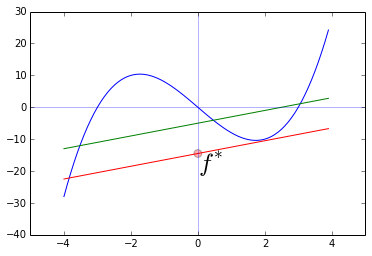
\includegraphics[width=0.5\textwidth]{./conj.png}}
\end{center}
(b)
\begin{align*}
&f^*(\lambda\bm \mu_1+(1- \lambda )\bm \mu_2)
\\
=&\inf\{f(\bm x)-\lambda\bm \mu_1^T\bm x+(1- \lambda )\bm \mu_2^T\bm x\}
\\
=&\inf\{f(\bm x)-\lambda\bm \mu_1^T\bm x+(1- \lambda )\bm \mu_2^T\bm x\}
\\
=&
\inf\{\lambda(f(\bm x)-\bm \mu_1^T\bm x)+(1- \lambda )(f(\bm x)-\bm \mu_2^T\bm x)\}
\\
\ge&
\inf\{\lambda\inf(f(\bm x)-\bm \mu_1^T\bm x)+(1- \lambda )\inf(f(\bm x)-\bm \mu_2^T\bm x)\}
\\
=&\inf\{\lambda f^*(\bm\mu_1) +(1- \lambda ) f^*(\bm\mu_2)\}
\\
\therefore&f^*(\lambda\bm \mu_1+(1- \lambda )\bm \mu_2)
>\inf\{\lambda f^*(\bm\mu_1) +(1- \lambda ) f^*(\bm\mu_2)\}
\\
\therefore&f^*\mathrm{\ is\ concave.}
\end{align*}
same method for $g_*(\mu)$

(c)
\begin{align*}
&\inf\left\{  f(\bm x) -g(\bm x):\bm x \right\}
\\
=&
\inf\left\{  f(\bm x)-\bm \mu^T\bm x -( g(\bm x)-\bm \mu^T\bm x ):\bm x \right\}
\\
\ge&
\inf\left\{  f(\bm x)-\bm \mu^T\bm x :\bm x\right\}+
\inf\left\{-( g(\bm x)+\bm \mu^T\bm x ):\bm x \right\} 
\mathrm{\ stands\ for\ all\ }\bm\mu
\\
\therefore&
\inf\left\{  f(\bm x) -g(\bm x):\bm x \right\}
\ge\sup\left\{ \inf\left\{  f(\bm x)-\bm \mu^T\bm x :\bm x\right\}-
\sup\left\{\bm \mu^T\bm x )-( g(\bm x):\bm x \right\} 
\right\}
\\
&\inf\left\{  f(\bm x) -g(\bm x):\bm x \right\}
\ge\sup\left\{
 f^*(\bm \mu) -g^*(\bm \mu)  \right\}
\end{align*}

(d,e)
\begin{align*}
    \min_x  f(\bm x) -g(\bm x)
    \\
-f(\bm x)+\bm \mu^T\bm x +f^*(\bm \mu)&\le0
\\
g(\bm x)-\bm \mu^T\bm x-g^*(\bm \mu)&\le0
\end{align*}

Dual:
\begin{align*}
    \max  &\theta(\bm v)
    \\
    \bm v\ge&0
    \\\theta(\bm v) =&\inf\left\{ f(\bm x) -g(\bm x)
    +
    \bm v_1(
-f(\bm x)+\bm \mu^T\bm x +f^*(\bm \mu))+
    \bm v_2(
g(\bm x)-\bm \mu^T\bm x-g^*(\bm \mu)
):\bm x\right\}
    \\\theta(\bm v) =&v_1f^*(\bm \mu)-v_2g^*(\bm \mu)
    +\inf\left\{ 
     (v_1-1)(
-f(\bm x)+\bm \mu^T\bm x )+
    (v_2-1)(
g(\bm x)-\bm \mu^T\bm x)
):\bm x\right\}
    \\\max\theta(\bm v) =&f^*(\bm \mu)-g^*(\bm \mu)
    ,\\
    \inf(f(\bm x)-g(\bm x))=&\sup(f^*(\bm \mu)-g^*(\bm \mu)) (\because 
    f-g,f^*-g^*\mathrm{ \  are\ convex,\  Strong\  Duality\  Theorem })
\end{align*}
\section*{7.24}
(a)
\begin{align*}
    \min -3x_1-2x_2&\\
    s.t. -x_1^2+x_2+1&\le0\\
    2x_1+3x_2&\le 6\\
    x_1,x_2&\ge0
\end{align*}

\begin{align*}
    \min -3x_1-2x_2&\\
    s.t. -x_1^2+x_2+1&\le0\\
    \begin{bmatrix}
        2&3\\
        -1&-1
    \end{bmatrix}
   \bm x \le
   \begin{bmatrix}
        6\\
        0
    \end{bmatrix}
\end{align*}
\begin{lstlisting}
Initial:
Z_1=Polyhedron({0,2},({0,-2},{1.5,1})
Step 1:
linear programming result: x_1={1.5,1}
g(x_1)>0
Step 2: 
barx_1={1.430,1.046}
Z_2=Polyhedron({0,2},({0,-2},{1.2139,0.4279},{1.430,1.046})
Step 1:
linear programming result: x_2={1.430,1.046}
g(x_2)<=0
Result:{1.430,1.046}
\end{lstlisting}
\begin{center}
\mbox{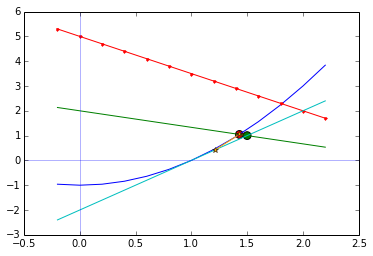
\includegraphics[width=0.3\textwidth]{./cut.png}}
\end{center}

(b)$B$ should be pseudo-convex to facilitate slacking into linear programming 
problem.

(c)
\begin{enumerate}
    \item 
$\left\{\bm x \right\}$ $\left\{\bm{\bar x } \right\}$ are in the $R^q, R^r$ respectively.
\item 
    For all Z, if $\bm x\in \bm f(Z)$, $\bm x\in Z$
\item 
    G is a closed map
\item 
    Given $\bm x \not\in \{g(x)\le0\} and Z, where \bm x \in 
\bm f(Z),
\bm{\bar x } \in {g(x)\le0} $, implying that 
$x\not\in\bm\nabla g(\bm{\bar x})(\bm x-\bm{\bar x})\ge0$
and 
$Z\cap\{\bm x:\bm\nabla g(\bm{\bar x})(\bm x-\bm{\bar x})\ge0\}\neq $\O
\end{enumerate}
For any k, we have
$\bm\nabla g(\bm{\bar x_k})(\bm x_l-\bm{\bar x_k})\ge0$, $l\ge k+1$
Before we end the program, we would have
$\bm\nabla g(\bm{\bar x})(\bm x-\bm{\bar x})\ge0$.
$\therefore\bm x \in \{g(x)\le0\}$, it is the optimal.

\section*{8.60}
$\bm{\bar x}=(-2,3,1,2)^T$,
$X=\{\bm x:\bm x^T\bm 1=1, \bm0\le\bm x\le\bm 1\}$.

Initialization: set $( \bm{\bar x^0},\bm I^0, \bm l^0, \bm \mu^0, \beta^0 )
= ( (-2,3,1,2)^T,\{1,2,3,4\}, \bm 0, \bm 1, 1 )$

Step 1:
\begin{align*}
\hat{x}_i^0 = \bar x_i^0+\frac{1-4}{4}*1
\\
\hat{\bm x}^0= \bm{\bar x}^0-3/4\bm1=(-2.75,2.25,0.25,1.25 )
\end{align*}

Step 2:
\begin{align*}
 \gamma=1+2.75+1.5=5.25>\beta \\
 J_3=\{1\}, J_4=\emptyset \\
x^*_1=0\\
I^{2}={2,3,4}\\
( \bm{\bar x^1},\bm I^1, \bm l^1, \bm \mu^1, \beta^1 )
= ( (3,1,2)^T,\{2,3,4\}, \bm 0, (1,0.25,1), 1 )
\end{align*}

Step 1:
\begin{align*}
\hat{\bm x}^1= (3,1,2)^T+\frac{1-6}{3}*1
=(\frac{4}{3},-\frac{2}{3},\frac{1}{3})
\end{align*}

Step 2:
\begin{align*}
 \gamma_1=1+\frac{2}{3}+\frac{1}{3} =2>\beta \\
 J_3=\{3\}, J_4=\emptyset \\
x^*_3=0\\
I^{1}={2,4}\\
( \bm{\bar x^2},\bm I^2, \bm l^2, \bm \mu^2, \beta^2 )
= ( (\frac{4}{3},\frac{1}{3})^T,\{2,4\}, \bm 0, (1,\frac{1}{3}), 1 )
\end{align*}

Step 1:
\begin{align*}
\hat{\bm x}^2= (\frac{4}{3},\frac{1}{3})^T-\frac{1}{3}\bm 1
=(1,0)
\end{align*}

Result:
$x^*=(0,1,0,0)$

\end{document}
